\section{Lebar, Tinggi, dan box-sizing}

Properti \code{width} dan \code{height} mengatur dimensi area content elemen. Nilai dapat berupa satuan absolut (px), relatif (em, rem, \%), atau keyword seperti \code{auto} (browser menghitung secara otomatis). Untuk layout yang fleksibel, properti \code{min-width}, \code{max-width}, \code{min-height}, dan \code{max-height} membatasi ukuran elemen agar tetap responsif---misalnya, \code{max-width: 800px;} memastikan elemen tidak melebihi 800px meskipun kontainernya lebih lebar \cite{mdnCss}.

Properti \textbf{box-sizing} mengontrol cara browser menghitung dimensi total elemen. Terdapat dua model: \code{content-box} (default) dan \code{border-box}. Perbedaan keduanya sangat signifikan dan sering menjadi sumber kebingungan bagi pemula. Memahami box-sizing adalah langkah kritis untuk menghasilkan layout yang presisi dan mudah diprediksi \cite{webdevCss}.

\begin{figure}[htbp]
\centering
\resizebox{\textwidth}{!}{%
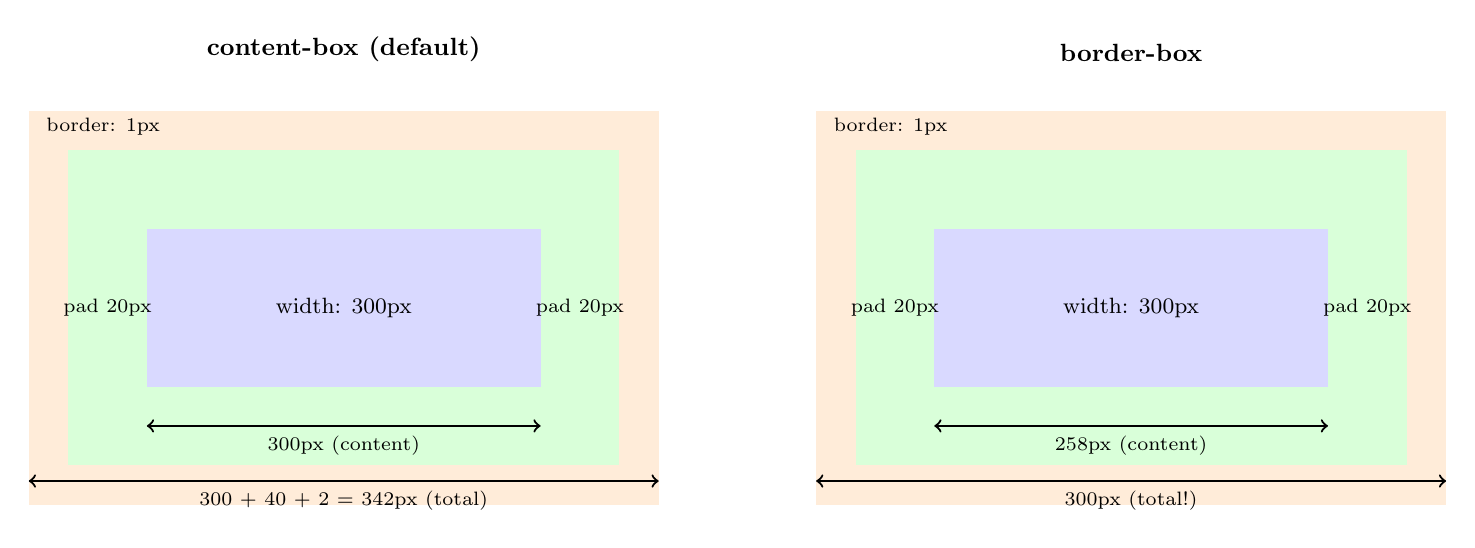
\begin{tikzpicture}[every node/.style={font=\footnotesize}]
  % content-box
  \node[font=\bfseries\small, anchor=south] at (4,5.5) {content-box (default)};
  \fill[orange!15] (0,0) rectangle (8,5);
  \fill[green!15] (0.5,0.5) rectangle (7.5,4.5);
  \fill[blue!15] (1.5,1.5) rectangle (6.5,3.5);
  \node at (4,2.5) {\code{width: 300px}};
  \draw[<->, thick] (1.5,1) -- node[below, font=\scriptsize] {300px (content)} (6.5,1);
  \draw[<->, thick] (0,0.3) -- node[below, font=\scriptsize] {300 + 40 + 2 = 342px (total)} (8,0.3);
  \node[font=\scriptsize] at (1,2.5) {pad 20px};
  \node[font=\scriptsize] at (7,2.5) {pad 20px};
  \node[font=\scriptsize, anchor=west] at (0.1,4.8) {border: 1px};

  % border-box
  \node[font=\bfseries\small, anchor=south] at (14,5.5) {border-box};
  \fill[orange!15] (10,0) rectangle (18,5);
  \fill[green!15] (10.5,0.5) rectangle (17.5,4.5);
  \fill[blue!15] (11.5,1.5) rectangle (16.5,3.5);
  \node at (14,2.5) {\code{width: 300px}};
  \draw[<->, thick] (10,0.3) -- node[below, font=\scriptsize] {300px (total!)} (18,0.3);
  \draw[<->, thick] (11.5,1) -- node[below, font=\scriptsize] {258px (content)} (16.5,1);
  \node[font=\scriptsize] at (11,2.5) {pad 20px};
  \node[font=\scriptsize] at (17,2.5) {pad 20px};
  \node[font=\scriptsize, anchor=west] at (10.1,4.8) {border: 1px};
\end{tikzpicture}%
}
\caption{Perbandingan content-box vs border-box: cara perhitungan width}
\end{figure}

Pada \code{content-box}, properti \code{width} dan \code{height} hanya berlaku untuk area content. Padding dan border \textbf{ditambahkan} di luar ukuran tersebut. Artinya, jika \code{width: 300px}, \code{padding: 20px}, dan \code{border: 1px}, total lebar visual elemen menjadi $300 + 20 \times 2 + 1 \times 2 = 342$ px. Ini membuat kalkulasi layout menjadi rumit karena setiap perubahan padding atau border mengubah total dimensi elemen \cite{cssTricks}.

Pada \code{border-box}, properti \code{width} dan \code{height} mencakup content \textbf{plus} padding \textbf{plus} border. Jika \code{width: 300px}, maka total lebar visual elemen tetap 300px---browser secara otomatis mengurangi area content untuk mengakomodasi padding dan border. Model ini membuat layout jauh lebih mudah diprediksi dan menjadi praktik standar di hampir semua framework CSS modern. Rekomendasi: terapkan \code{border-box} secara global \cite{webdevCss}.

Properti \code{overflow} mengontrol perilaku ketika konten melebihi dimensi elemen. Nilai \code{visible} (default) membiarkan konten meluap keluar kotak. \code{hidden} memotong konten yang meluap. \code{scroll} selalu menampilkan scrollbar. \code{auto} menampilkan scrollbar hanya jika konten meluap. Untuk layout modern, \code{overflow: hidden;} sering digunakan pada kontainer untuk mencegah tata letak yang rusak \cite{mdnCss}.

\begin{webcode}[language=CSS, caption={box-sizing global dan overflow}]
/* Reset global: border-box untuk semua elemen */
*, *::before, *::after {
  box-sizing: border-box;
}

/* Kotak dengan kalkulasi mudah */
.sidebar {
  width: 25%;       /* 25% dari parent */
  padding: 16px;    /* termasuk dalam 25% */
  border: 1px solid #ccc;
}

/* Kontainer dengan min/max dan overflow */
.container {
  width: 100%;
  max-width: 1200px;
  min-height: 400px;
  margin: 0 auto;
  overflow: auto;   /* scrollbar jika konten meluap */
}
\end{webcode}

\begin{konsep}
\textbf{Selalu Gunakan \code{border-box} Secara Global.} Praktik modern yang diadopsi oleh hampir semua framework CSS (Bootstrap, Tailwind, dll.) adalah menerapkan \code{box-sizing: border-box} pada semua elemen. Ini menghilangkan kebingungan perhitungan ukuran dan membuat layout berbasis persentase jauh lebih mudah. Selalu letakkan reset \code{*, *::before, *::after \{ box-sizing: border-box; \}} di awal stylesheet Anda \cite{cssTricks}.
\end{konsep}

